\documentclass{beamer}
\usepackage{tcolorbox}
\ProvidesPackage{notation}
\RequirePackage{tcolorbox}
\RequirePackage{bm}
\usepackage{amsmath}
\usepackage{tikz}
\usepackage{pgfplots}
\usepackage{adjustbox}
\usepackage{calculator}
\usetikzlibrary{calc}

\pgfplotsset{compat=1.14}

% Draw vector and corresponding unitvector
\newcommand{\vecuvec}[2] %start point, end point (of vector)
{   \VECTORSUB(#2)(#1)(\sola,\solb,\solc)
	\UNITVECTOR(\sola, \solb, \solc)(\sola,\solb,\solc)
	%arrow in blue
	\draw[->,thick,blue] (#1) -- (#2); 
	%corresponding unit-vector in red:
	\edef\temp{\noexpand\draw[->, thick,red] (#1) -- ($(#1)+(\sola,\solb,\solc)$);}
	\temp
}


%\beamerdefaultoverlayspecification{<+->}
\newcommand{\data}{\mathcal{D}}

\DeclareMathOperator*{\argmin}{arg\,min}

\newcommand\Item[1][]{%
	\ifx\relax#1\relax  \item \else \item[#1] \fi
	\abovedisplayskip=0pt\abovedisplayshortskip=0pt~\vspace*{-\baselineskip}}


\usetheme{metropolis}           % Use metropolis theme


\title{Geometric Interpretation of Linear Regression}
\date{\today}
\author{Nipun Batra}
\institute{IIT Gandhinagar}
\begin{document}
	\maketitle
	
	
	\begin{frame}{Linear Combination of Vectors}
		Let $v_{1},v_{2},v_{3},\dots,v_{i}$ be vectors in  ${\rm I\!R}^{D}$, where $D$ denotes the dimensions. \pause \\A linear combination of $v_{1},v_{2},v_{3},\dots,v_{i}$ is of the following form
		
		\pause \begin{equation*}
			\alpha_{1}v_{1}+			\alpha_{2}v_{2}+			\alpha_{3}v_{3}+
			\dots+\alpha_{i}v_{i}
		\end{equation*}
		
		where $\alpha_{1},\alpha_{2},\alpha_{3},\dots,\alpha_{i} \in {\rm I\!R}$
		
	\end{frame}

\begin{frame}{Span of vectors}
		Let $v_{1},v_{2},\dots,v_{i}$ be vectors in  ${\rm I\!R}^{D}$, with $D$ dimensions. \\
		\pause The span of  $v_{1},v_{2},\dots,v_{i}$ is denoted by SPAN\{$v_{1},v_{2},\dots,v_{i} $\}
		
		\pause \begin{equation*}
	    \{	\alpha_{1}v_{1}+			\alpha_{2}v_{2}+
		\dots+\alpha_{i}v_{i} \hspace{1em}\vert \hspace{1em}  \alpha_{1},\alpha_{2},\dots,\alpha_{i} \in {\rm I\!R}\}
		\end{equation*}
		
		\pause  It is the set of all vectors that can be generated by linear combinations of $v_{1},v_{2},\dots,v_{i}$.
\end{frame}

\begin{frame}{Example}
Find the span of ($\begin{bmatrix}
1 \\2
\end{bmatrix}, \begin{bmatrix}
2 \\1
\end{bmatrix}) $

\pause \begin{tikzpicture}
\begin{axis}
[
axis x line  = bottom,
axis y line  = left,
ymax         = 4,
ymin         = -2,
xmax         = 4,
xmin         = -2,
]
\node[anchor=west] (A) at (axis cs:1,2){$v_1$};
\node (B) at (axis cs:2,1){$v_2$};
\node (D) at (axis cs:0, 0){};

\draw[->](D)--(A);
\draw[->](D)--(B);
\end{axis}

\end{tikzpicture}



\end{frame}

\begin{frame}{Example}

\begin{tikzpicture}
\begin{axis}
[
axis x line  = bottom,
axis y line  = left,
ymax         = 4,
ymin         = -1,
xmax         = 4,
xmin         = -1,
]
\node[anchor=west] (A) at (axis cs:1,2){$v_1$};
\node (B) at (axis cs:2,1){$v_2$};
\node (D) at (axis cs:0, 0){};

\node (v3) at (axis cs:3,3){$v_3$};
\node (v4) at (axis cs:-1,1){$v_4$};
\draw[->](D)--(A);
\draw[->](D)--(B);
\draw[->](D)--(v3);
\draw[->](D)--(v4);
\end{axis}

\end{tikzpicture}

$v_3 = v_1 + v_2$ and $v_4 = v_1 - v_2$

Span(($v_1, v_2$)) $\in \mathcal{R}^2$ 
\end{frame}


\begin{frame}{Example}
Find the span of ($\begin{bmatrix}
1 \\2
\end{bmatrix}, \begin{bmatrix}
2 \\4
\end{bmatrix}) $

\pause Can we obtain a point (x, y) s.t. x = 3y? \\
\pause No \\ 
\pause Span of the above set is along the line y = 2x

\end{frame}

\begin{frame}{Example}
Find the span of ($\begin{bmatrix}
1 \\1\\1
\end{bmatrix}, \begin{bmatrix}
2 \\-2\\2
\end{bmatrix}) $
\pause \begin{adjustbox}{max totalsize={0.4\textwidth},center}
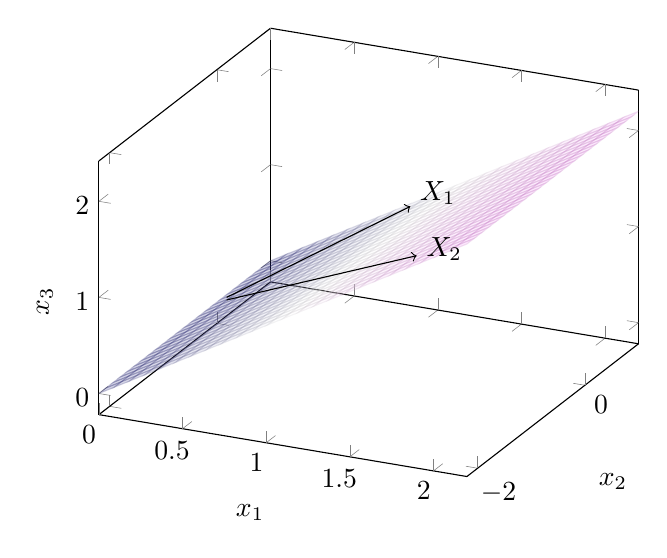
\begin{tikzpicture}
\begin{axis}[xlabel=$x_1$, ylabel=$x_2$, zlabel=$x_3$]
\addplot3[
surf,
domain=0:2.2,
y domain=-2.2:1,
colormap/violet,
opacity=0.2,
]
{x};

%\node{D}  at (axis cs:0, 0, 0){};
\node (A) at (axis cs:1, 1, 1) {$X_1$};
\node (D) at (axis cs:0,0,0) {};
\node (B) at (axis cs:2, -2, 2) {$X_2$};

\draw[->] (D) -- (A);
\draw[->] (D) -- (B);



%	\addplot3 coordinates {
%	(8.89, 0.61, 1.77)
%	(5.33, 0.61, 5.33)
%};

\end{axis}
\end{tikzpicture}
\end{adjustbox}
\pause The span is the plane $z=x$ or $x_3=x_1$
\end{frame}

\begin{frame}{Geometric Interpretation}
Consider $X$ and $y$ as follows. 
$$
\mathbf{X}=\left(\begin{array}{cc}
{1} & {2} \\
{1} & {-2} \\
{1} & {2}
\end{array}\right), \quad \mathbf{y}=\left(\begin{array}{c}
{8.8957} \\
{0.6130} \\
{1.7761}
\end{array}\right)
$$
\begin{itemize}[<+->]
	\item We are trying to learn $\theta$ for $\hat{y}=X\theta$ such that $\vert \vert y - \hat{y} \vert \vert_{2}$ is minimised
	\item Consider the two columns of X. Can we write $X\theta$ as the span of ($\begin{bmatrix}
	1 \\1\\1
	\end{bmatrix}, \begin{bmatrix}
	2 \\-2\\2
	\end{bmatrix}$)?
	\item We wish to find $\hat{y}$ such that 
	$$
	\underset{\hat{y} \in SPAN\{\bar{x_{1}},\bar{x_{2}},\dots,\bar{x_{D}}\} } \argmin \vert \vert y - \hat{y} \vert \vert_{2}
	$$
\end{itemize}

\end{frame}


\begin{frame}{Geometric Interpretation}
Span of ($\begin{bmatrix}
1 \\1\\1
\end{bmatrix}, \begin{bmatrix}
2 \\-2\\2
\end{bmatrix}) $
\pause \begin{adjustbox}{max totalsize={0.4\textwidth},center}
	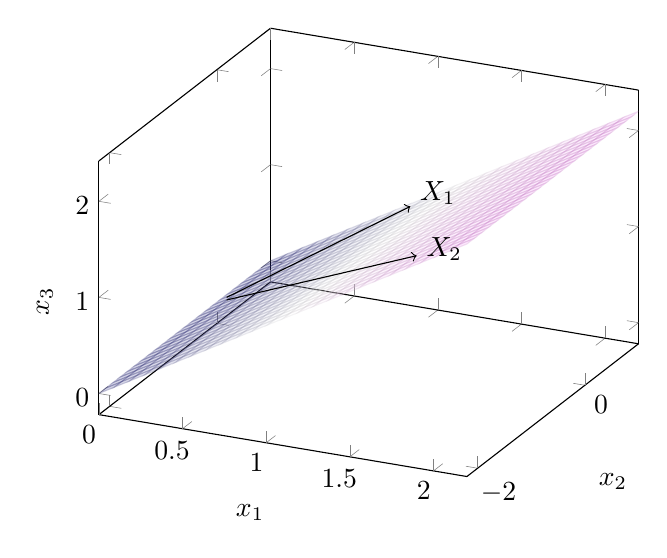
\begin{tikzpicture}
	\begin{axis}[xlabel=$x_1$, ylabel=$x_2$, zlabel=$x_3$]
	\addplot3[
	surf,
	domain=0:2.2,
	y domain=-2.2:1,
	colormap/violet,
	opacity=0.2,
	]
	{x};
	
	%\node{D}  at (axis cs:0, 0, 0){};
	\node (A) at (axis cs:1, 1, 1) {$X_1$};
	\node (D) at (axis cs:0,0,0) {};
	\node (B) at (axis cs:2, -2, 2) {$X_2$};
	
	\draw[->] (D) -- (A);
	\draw[->] (D) -- (B);
	
	
	
	%	\addplot3 coordinates {
	%	(8.89, 0.61, 1.77)
	%	(5.33, 0.61, 5.33)
	%};
	
	\end{axis}
	\end{tikzpicture}
\end{adjustbox}
The span is the plane $z=x$ or $x_3=x_1$
\end{frame}


\begin{frame}{Geometric Interpretation}	

		\begin{adjustbox}{max totalsize={0.6\textwidth},center}
			
			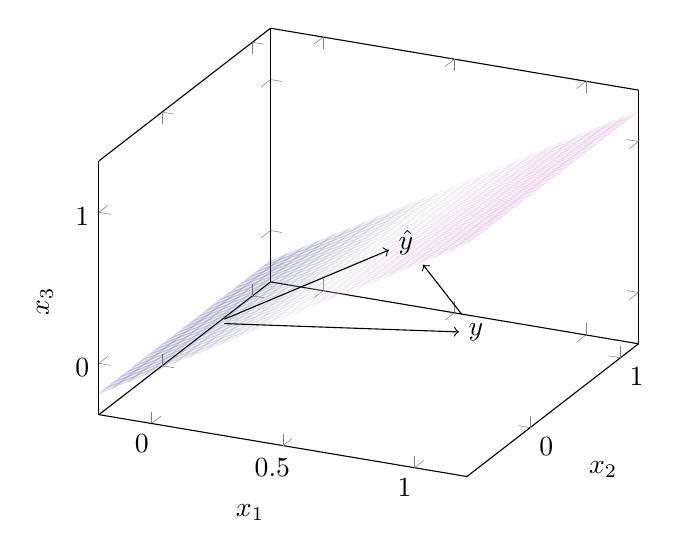
\begin{tikzpicture}
			\begin{axis}[xlabel=$x_1$, ylabel=$x_2$, zlabel=$x_3$]
			\addplot3[
			surf,
			domain=-0.2:1.2,
			y domain=-0.7:1.2,
			colormap/violet,
			opacity=0.1,
			]
			{x};
			
			%\node{D}  at (axis cs:0, 0, 0){};
			
			\node (D) at (axis cs:0,0,0) {};
			
			\node (C) at (axis cs:0.97, 0.07, 0.19) {$y$};
			\node (E) at (axis cs:0.70, 0.08, 0.70) {$\hat{y}$};
			\draw[->] (D) -- (C);
			\draw[->] (D) -- (E);
			\draw[->] (C) -- (E);
			
			
			%	\addplot3 coordinates {
			%	(8.89, 0.61, 1.77)
			%	(5.33, 0.61, 5.33)
			%};
			
			\end{axis}
			\end{tikzpicture}
		\end{adjustbox}
		


\begin{itemize}[<+->]
	\item We seek a $\hat{y}$ in the span of the columns of $X$ such that it is closest to $y$
	\item This happens when $y-\hat{y}\perp x_j \forall j$ or $x_j^T(y-\hat{y})=0$
	\item $X^T(y-X\theta)=0$
	\item $X^Ty = X^TX\theta$ or $\hat{\theta} =(X^TX)^{-1}X^Ty$ 
\end{itemize}

\end{frame}


%
%\begin{frame}{Subspace}
%	A subset $S$ $\in {\rm I\!R}$ is called a subspace if  
%	\begin{itemize}[<+->]
%		\item origin belongs to $S$
%		\item if $u,v \in S$, then $u+v \in S$  
%		\item if $u \in S$, then $\alpha u \in S$,  $\forall \alpha \in {\rm I\!R}$
%	\end{itemize}	
%\end{frame}
%
%\begin{frame}{When does a Span become a subspace?}
%	Think about it!
%\end{frame}
%
%
%
%\begin{frame}{}	\begin{columns}
%	\pause \begin{column}{0.6\textwidth}
%		\begin{adjustbox}{max totalsize={\textwidth},center}
%			
%			\begin{tikzpicture}
%			\begin{axis}[xlabel=$x_1$, ylabel=$x_2$, zlabel=$x_3$,title={Surface Plot}]
%			\addplot3[
%			surf,
%			domain=0:2.2,
%			y domain=-2.2:1,
%			colormap/violet,
%			opacity=0.2,
%			]
%			{x};
%			
%			%\node{D}  at (axis cs:0, 0, 0){};
%			\node (A) at (axis cs:1, 1, 1) {$X_1$};
%			\node (D) at (axis cs:0,0,0) {};
%			\node (B) at (axis cs:2, -2, 2) {$X_2$};
%			
%			\draw[->] (D) -- (A);
%			\draw[->] (D) -- (B);
%
%			
%			
%			%	\addplot3 coordinates {
%			%	(8.89, 0.61, 1.77)
%			%	(5.33, 0.61, 5.33)
%			%};
%			
%			\end{axis}
%			\end{tikzpicture}
%		\end{adjustbox}
%		
%	\end{column}
%\end{columns}
%\end{frame}
%
%
%
%
%
%\begin{frame}
%Solution: 2.97, 1.18
%0.97853679, 0.06714369, 0.19482678
%
%$$x_1 = (1, 1, 1)/||<1, 1, 1>||$$
%
%0.58, 0.58, 0.58
%
%
%Solution: 5.33, 0.61, 5.33 to .70480267, 0.08066222, 0.70480267
%\end{frame}
%
%\begin{frame}
%\begin{tikzpicture}
%\draw[->](0,0) -- (5,0);
%\end{tikzpicture}
%
%\begin{tikzpicture}
%\draw[<<->>](0,0) -- (5,0);
%\end{tikzpicture}
%
%\begin{tikzpicture}
%\draw[<<->>, ultra thick, blue](0,0) -- (5,0);
%\end{tikzpicture}
%
%\begin{tikzpicture}
%\draw[|->>, thick, red](0,0) -- (5,0);
%\end{tikzpicture}
%
%
%
%\end{frame}
%	


%\begin{frame}{Geometric Interpretation of Linear Regression}
%	Let $\bar{x_{j}}$ denote the $j^{th}$ column of $X$. \\
%	Let $\hat{y}$ be the prediction.
%	
%	$$
%	\hat{y} = w_{1}\bar{x_{1}}+w_{2}\bar{x_{2}}+\dots+w_{D}\bar{x_{D}} = XW
%	$$
%	
%	
%	Clearly, $\hat{y} \in $ SPAN\{$\bar{x_{1}},\bar{x_{2}},\dots,\bar{x_{D}}$\} 
%	How to choose the best $\hat{y}$?
%\end{frame}
%
%\begin{frame}{Geometric Interpretation of Linear Regression}
%	We wish to $\hat{y}$ such that 
%	$$
%		\underset{\hat{y} \in SPAN\{\bar{x_{1}},\bar{x_{2}},\dots,\bar{x_{D}}\} } \argmin \vert \vert y - \hat{y} \vert \vert_{2}
%	$$
%\end{frame}

%\begin{frame}{Geometric Interpretation of Linear Regression}
%	It is analogus to choosing $\hat_{y}$ such that it is closest to $y$. It is the projection of $y$ onto the column space of $X$.
%	\vspace{2em}\\
%	Hence the residual vector $y - \hat{y}$ will be perpendicular to each of the columns of $X$. 
%\end{frame}


%
%\begin{frame}{Geometric Interpretation of Linear Regression}
%	$$
%		\bar{x_{i}}(y - \hat{y}) = 0
%	$$
%	
%	$$
%		X^{T}(y - XW) = \mathbf{0}
%	$$
%	
%	\begin{tcolorbox}
%		$$
%			W = (X^{T}X)^{-1}X^{T}y
%		$$
%	\end{tcolorbox}
%
%	
%	
%\end{frame}
%
%\begin{frame}
%\begin{tikzpicture}
%\begin{axis}
%\addplot3 coordinates {
%	(0.81,	0.19,	0.00)
%	(0.76,	0.17,	0.07)
%	(0.66,	0.16,	0.16)
%	(0.76,	0.07,	0.17)
%	(0.81,	0.00,	0.19)
%};
%
%\addplot3 coordinates {
%	(0.85,	0.15,	0.00)
%	(0.82,	0.13,	0.05)
%	(0.73,	0.14,	0.13)
%	(0.82,	0.06,	0.13)
%	(0.84,	0.00,	0.16)
%};
%
%\end{axis}
%\end{tikzpicture}
%\end{frame}



\end{document}